
\documentclass{beamer}
\usetheme{Madrid}
%\usetheme{Goettingen}
\usefonttheme{serif}
\usefonttheme{structuresmallcapsserif}
% \usepackage[font=small,labelfont=bf]{caption}
\usepackage{xcolor}
\usepackage{rotating}
\usepackage{multirow}
\usepackage{multicol}
\usepackage{soul}

\setbeamerfont{section title}{parent=title}
\setbeamercolor{section title}{parent=titlelike}
%\defbeamertemplate*{section page}{default}[1][]
%{
%    \centering
%    \begin{beamercolorbox}[sep=8pt,center,#1]{section title}
%        \usebeamerfont{section title}\insertsection\par
%    \end{beamercolorbox}
%}

\setbeamertemplate{navigation symbols}{}
%\newcommand*{\sectionpage}{\usebeamertemplate*{section page}}

\def\Put(#1,#2)#3{\leavevmode\makebox(0,0){\put(#1,#2){#3}}}

\makeatletter
\setbeamertemplate{footline}
{
    % Commented out to remove footer line entirely
%    \leavevmode%
%    \hbox{%
%    \begin{beamercolorbox}[wd=.333333\paperwidth,ht=2.25ex,dp=1ex,center]{author in head/foot}%
%        \usebeamerfont{author in head/foot}\insertshortauthor%~~\beamer@ifempty{\insertshortinstitute}{}{(\insertshortinstitute)}
%    \end{beamercolorbox}%
%    \begin{beamercolorbox}[wd=.333333\paperwidth,ht=2.25ex,dp=1ex,center]{title in head/foot}%
%        \usebeamerfont{title in head/foot}\insertshorttitle
%    \end{beamercolorbox}%
%    \begin{beamercolorbox}[wd=.333333\paperwidth,ht=2.25ex,dp=1ex,right]{date in head/foot}%
%        \usebeamerfont{date in head/foot}\insertshortdate{}\hspace*{2em}
%        \insertframenumber{} / \inserttotalframenumber\hspace*{2ex} 
%    \end{beamercolorbox}}%
%    \vskip0pt%
}
\makeatother

\newenvironment<>{varblock}[2][\textwidth]{
    \begin{center}
        \begin{minipage}{#1}
            \setlength{\textwidth}{#1}
            \begin{actionenv}#3
                \def\insertblocktitle{#2}
                \par
                \usebeamertemplate{block begin}}
            {\par
                \usebeamertemplate{block end}
            \end{actionenv}
        \end{minipage}
    \end{center}
}

\DeclareGraphicsExtensions{.pdf,.png,.jpg}

\setbeamerfont{section title}{parent=title}
\setbeamercolor{section title}{parent=titlelike}
\defbeamertemplate*{section page}{default}[1][]
{
      \centering
      \begin{beamercolorbox}[sep=8pt,center,#1]{section title}
          \usebeamerfont{section title}\insertsection\par
      \end{beamercolorbox}
}
\newcommand*{\sectionpage}{\usebeamertemplate*{section page}}


\begin{document}
\title{Ham Radio is for Nerds}
\subtitle{\ldots like me}
\author{Josh Tolley, KG7AKX}

{
    \usebackgroundtemplate{%
      \vbox to \paperheight{\vfil\hbox to \paperwidth{\hfil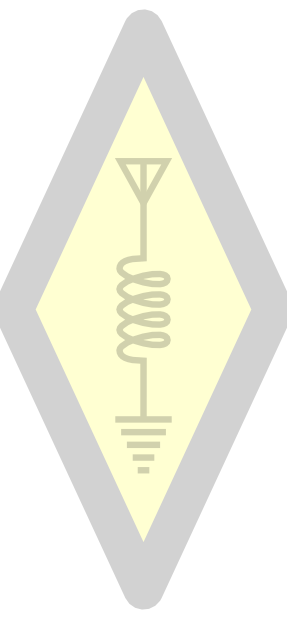
\includegraphics[height=\paperheight]{img/symbol-bkgrnd.png}\hfil}\vfil}
    }
    \begin{frame} 
        \titlepage 
    \end{frame} 
} 


% Ham radio used to be where aspiring hackers got started. Amateur radio is still
% a vibrant world with much to teach the interested geek. We'll talk about where
% ham radio fits in the hacker arsenal today, and cover everything you need to
% pass the FCC's licensing test and get on the air.

\section{Neat stuff radio can do}
{
    \usebackgroundtemplate{%
      \vbox to \paperheight{\vfil\hbox to \paperwidth{\hfil
\includegraphics[height=\paperheight]{img/omni-antenna.png}\hfil}\vfil}
    }
    \frame{\mysectionpage}
}

\begin{frame}{Neat stuff radio can do}
    \begin{columns}[onlytextwidth]
        \column{0.5\textwidth}
            \begin{itemize}
                \item \hilitem<1>{Communication between family and friends}
                \item \hilitem<2>{Emergency preparedness}
                \item \hilitem<3>{Alternative news and information sources}
                \item \hilitem<4>{Radio control devices}
                \item \hilitem<5>{Homebrew radar}
                \item \hilitem<6>{Wireless networking}
                \item \hilitem<7>{Aircraft and rocket avionics}
                \item \hilitem<8>{EME / Moonbounce, satellite, space station}
            \end{itemize}
        \column{0.5\textwidth}
            \centering
            \only<1>{
\includegraphics[width=0.9\textwidth]{img/family-friends.jpg} \\ }
            \only<2>{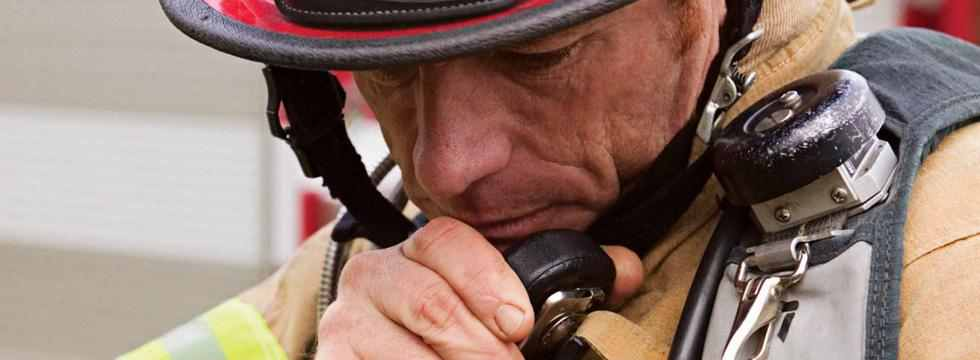
\includegraphics[width=0.9\textwidth]{img/emergency.png} \\ }
            \only<3>{
\includegraphics[width=0.9\textwidth]{img/news-info.jpg} \\ }
            \only<4>{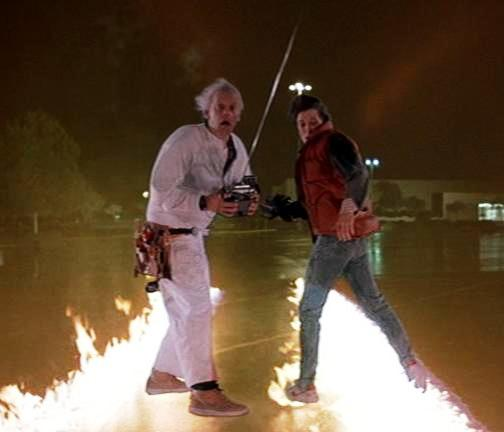
\includegraphics[width=0.9\textwidth]{img/radio-control.jpg} \\ }
            \only<5>{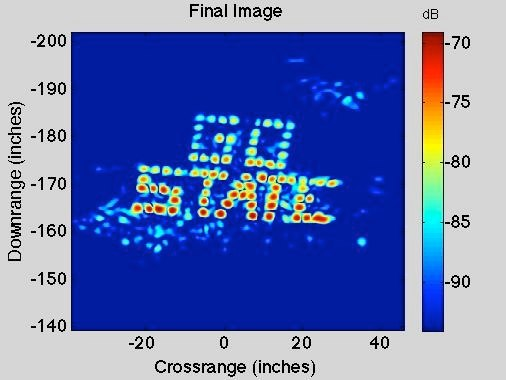
\includegraphics[width=0.9\textwidth]{img/radar.jpg} \\ }
            \only<6>{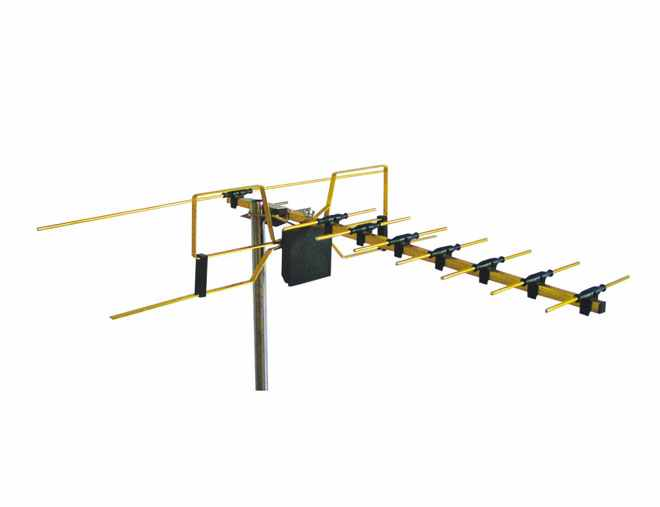
\includegraphics[width=0.9\textwidth]{img/networking.jpg} \\ }
            \only<7>{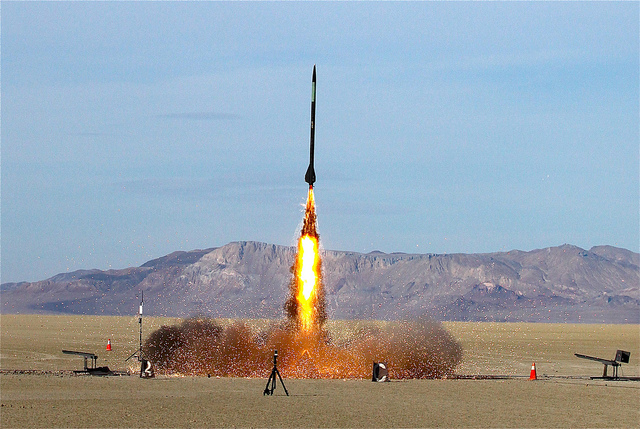
\includegraphics[width=0.9\textwidth]{img/avionics.jpg} \\  \tiny{Flickr user jurvetson} }
            \only<8>{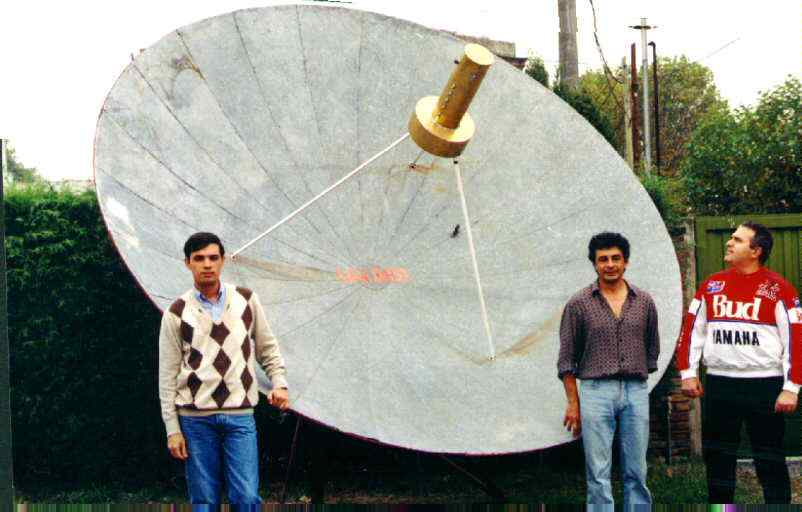
\includegraphics[width=0.9\textwidth]{img/eme.jpg} \\ }
    \end{columns}
\end{frame}

\section{How radio works}
{
    \usebackgroundtemplate{%
      \vbox to \paperwidth{\vfil\hbox to \paperwidth{\hfil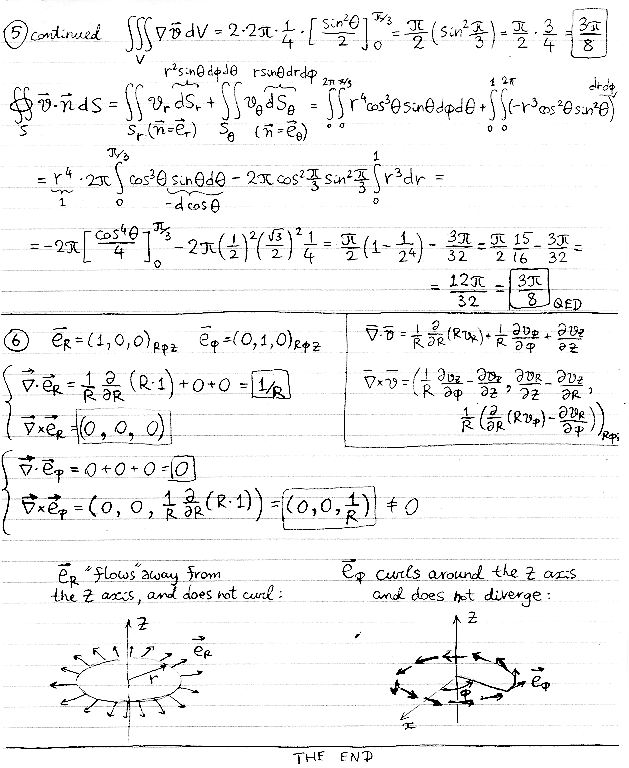
\includegraphics[width=\paperwidth]{img/vec_cal.png}\hfil}\vfil}
    }
    \frame{\mysectionpage}
}

\begin{frame}[t]{How radio works}
    \begin{multicols}{2}
        \begin{itemize}
            \item \hilitem<1>{Electric field}
            \item \hilitem<2>{Induction}
            \item \hilitem<3>{Carrier wave, frequency}
            \item \hilitem<4>{Modulation}
            \item \hilitem<5>{Amplification}
            \alt<6>{ \item Vector calculus }{ \item[] }
        \end{itemize}
    \end{multicols}
    \centering
    \only<1>{ 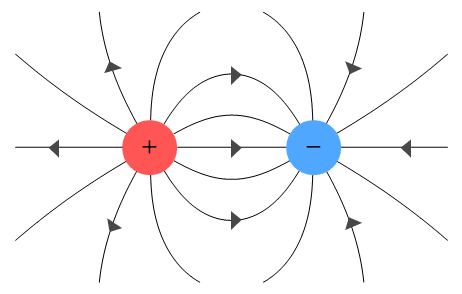
\includegraphics[height=0.6\textheight]{img/electric-field.png} \\}
    \only<2>{ 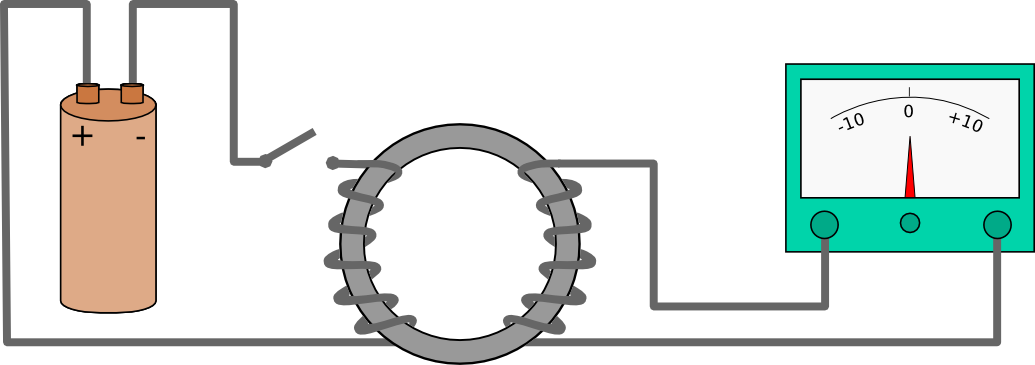
\includegraphics[width=0.9\textwidth]{img/induction.png} \\}
    \only<3>{ 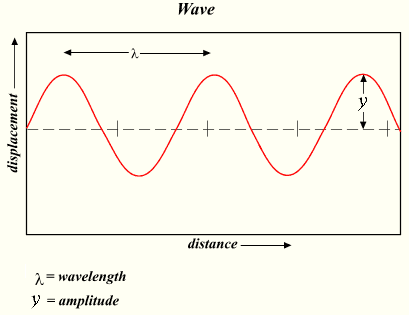
\includegraphics[height=0.6\textheight]{img/Wave.png} \\}
    \only<4>{ 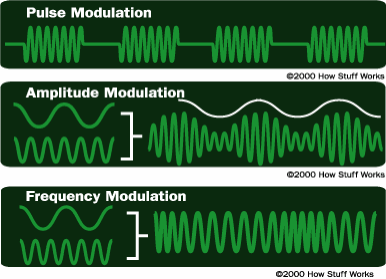
\includegraphics[height=0.6\textheight]{img/modulation.png} \\}
    \only<5>{ 
\includegraphics[height=0.6\textheight]{img/amplification.png} \\}
    \only<6>{ 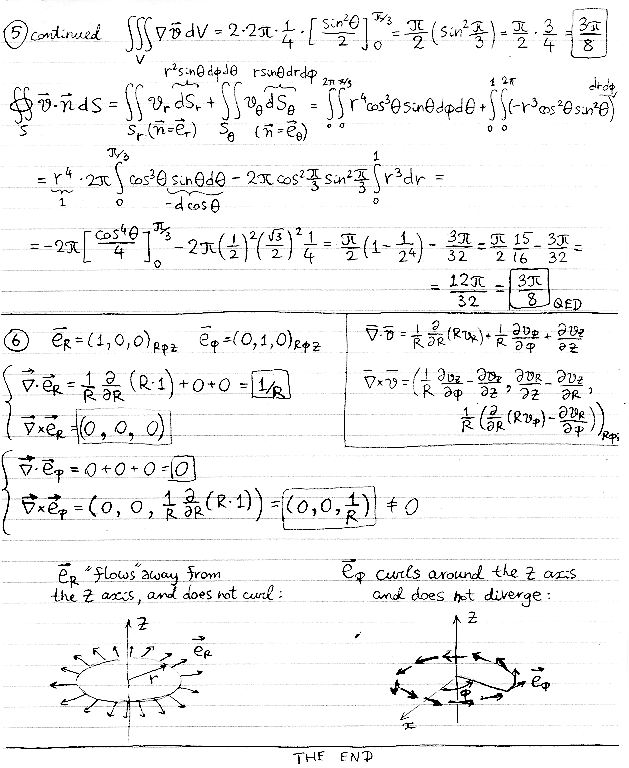
\includegraphics[height=0.6\textheight]{img/vec_cal.png} \\}
\end{frame}

\section{Ham radio specifics}
{
    %\usebackgroundtemplate{%
    %  \vbox to \paperwidth{\hbox to \paperwidth{\hfil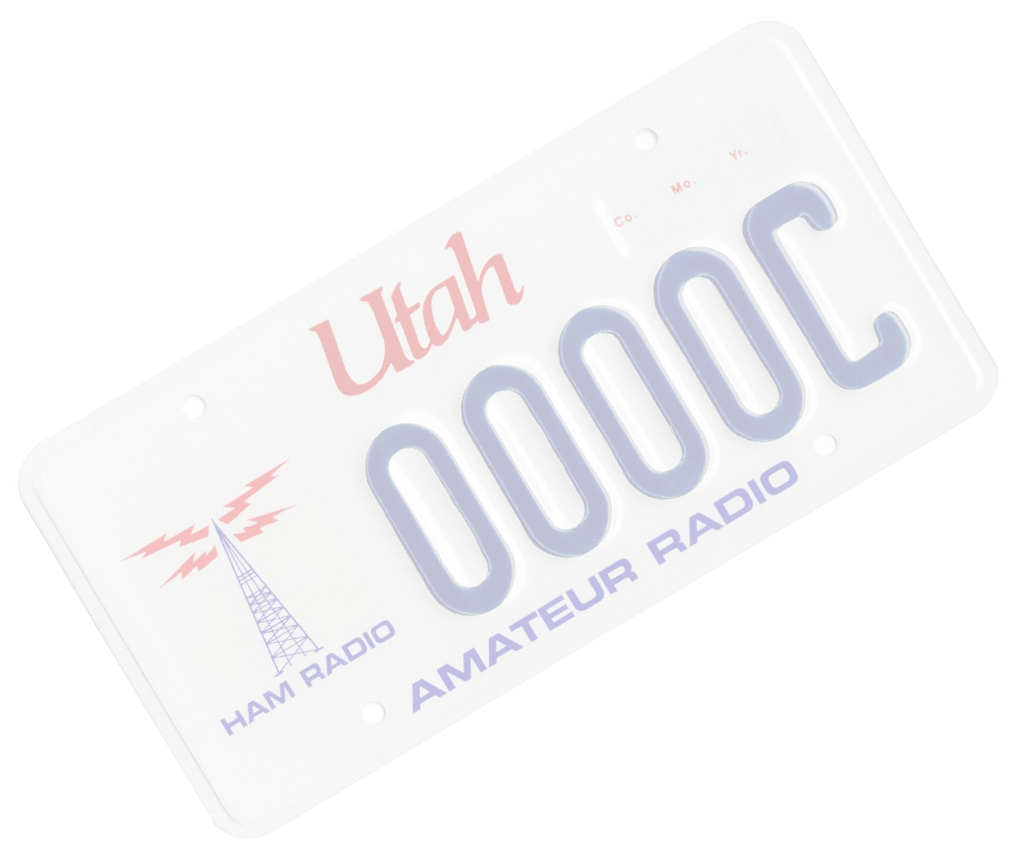
\includegraphics[width=\paperwidth]{img/utah-ham-plate-trans.png}\hfil}}
    %}
    \usebackgroundtemplate{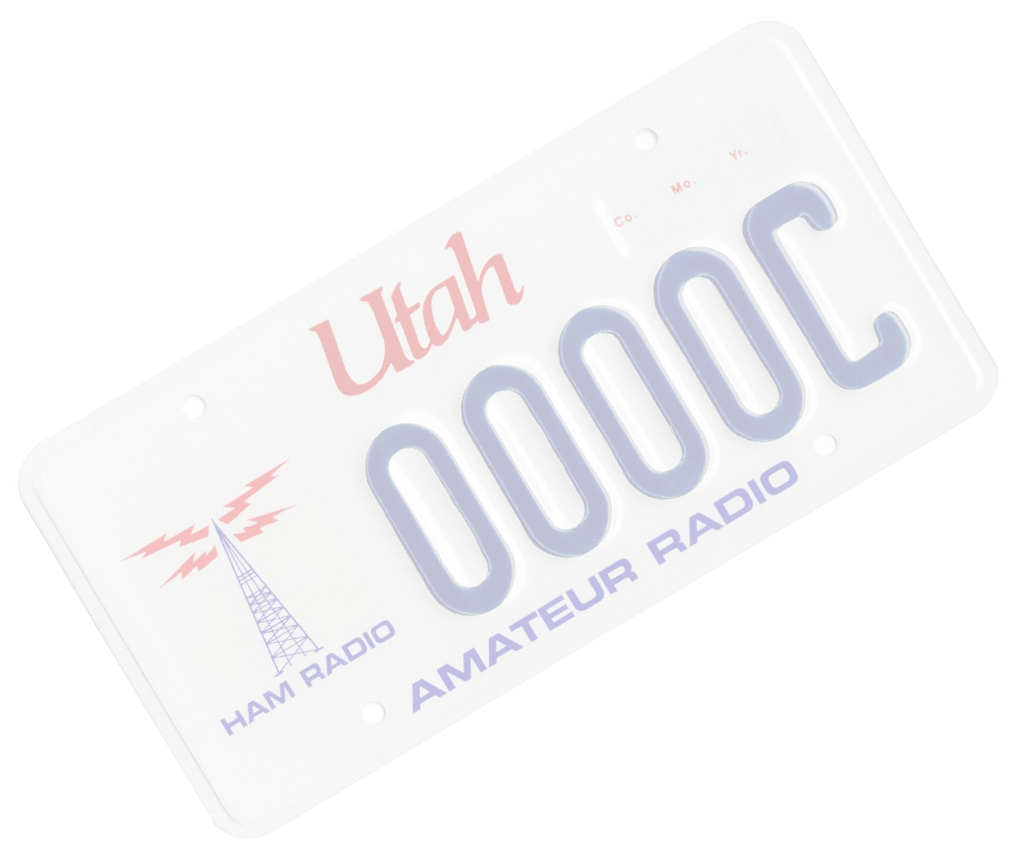
\includegraphics[width=\paperwidth]{img/utah-ham-plate-trans.png}}
    \frame{\mysectionpage}
}

\begin{frame}[t]{Ham radio}
    In the United States, the Federal Communications Commission regulates amateur radio by the following characteristics:
    \begin{multicols}{2}
        \begin{itemize}
            \item \hilitem<1>{Frequency}
            \item \hilitem<2>{Transmission power}
            \item \hilitem<3>{Mode}
            \item \hilitem<4>{``Communications decency''}
        \end{itemize}
    \end{multicols}
    \centering
    \only<1>{ 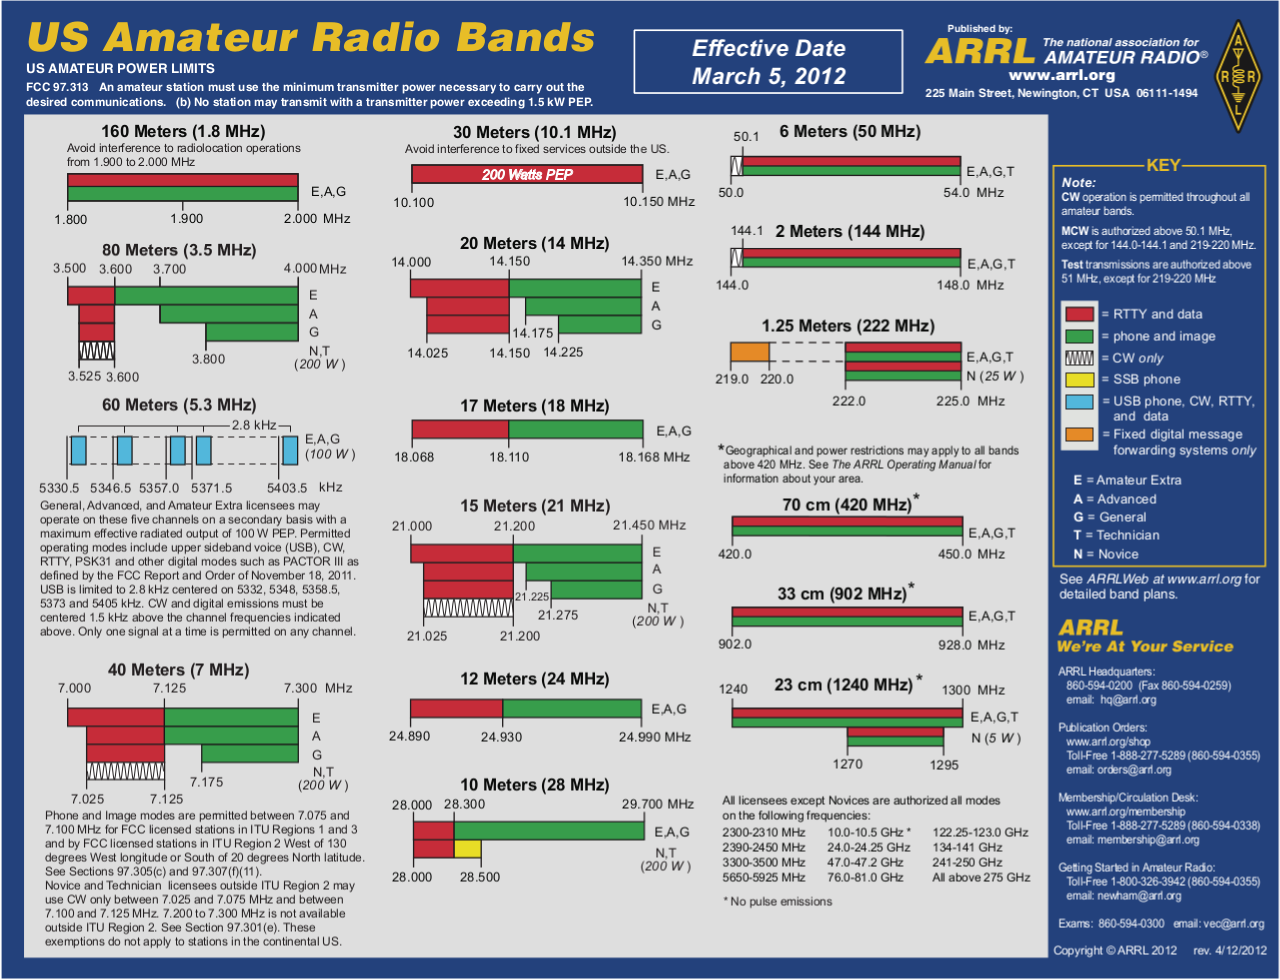
\includegraphics[height=0.5\textheight]{img/band-plan.png} \\ }
    \only<2>{ 
\includegraphics[height=0.5\textheight]{img/transmission-power.jpg} \\ }
    \only<3>{ 
\includegraphics[height=0.5\textheight]{img/language.png} \\ }
    \only<4>{ 
\includegraphics[height=0.5\textheight]{img/decency.jpg} \\ }
\end{frame}

\begin{frame}{Ham radio}
    \begin{varblock}[0.9\textwidth]{}
        \centering
        \huge{You need to %
        \only<1>{know }\only<2->{\st{know} have known }about all that stuff to transmit legally\only<3->{, or have gotten lucky on the test\only<4>{\textsuperscript{*}}}}\\
    \end{varblock}
    \vspace{3cm}
    \only<4>{\small{\textsuperscript{*} You can legally receive whatever you want. There's really no way they could stop you.}}
\end{frame}

\end{document}
